\section{Classification}
Our primary objective is to separate experimental data into two possible categories.
Supervised learning typically leverages large amounts of labeled data to learn
representations of the classes present in the inputs. A challenge in Physics is that
experiments generate enormous amounts of data, but it is not labeled. Hand-labeling
data is time-consuming and cost-ineffective. A possible solution to this challenge
is to train models on simulated data. The idea being that simulated and experimental
data are similar enough that the learned patterns from simulated data are, to some degree,
transferrable to experimental data.
The simulated data contains two classes of events - a single electron and a double electron.

\subsection{Simulated data}
In table \ref{tab:classification-simulated-f1} the performance of each model 
trained is reported using the f1-score. The model architecture for each model is described in (ref appendix).
As a benchmark, we are including a state of the art pretrained network (\cite{}VGG HERE) applied to the data 
using the approach described in \ref{section:method-pretrained}.
\begin{table}
\centering
\caption{
Mean F1-scores for classification of simulated data using multiple models. 
Error estimates are the standard deviation in results from k-fold cross-validation 
with $K=5$ folds.
}
\label{tab:classification-simulated-f1}
\begin{tabular}{llll}
\toprule
                                           Logistic &                                               Dense &                                       Convolutional &                                    Pretrained VGG16 \\
\midrule
 $\underset{\num{+- 7.727e-03 }  }{\num{ 0.734 } }$ &  $\underset{\num{+- 1.329e-02 }  }{\num{ 0.907 } }$ &  $\underset{\num{+- 6.286e-03 }  }{\num{ 0.959 } }$ &  $\underset{\num{+- 1.591e-02 }  }{\num{ 0.894 } }$ \\
\bottomrule
\end{tabular}
\end{table}

To give a broader picture of the performance we also include the calculated confusion matrix values in
table \ref{tab:classification-simulated-confmat}. Even if f1-scores are similar, there may still be differences
in either of the confusion matrix values.
\begin{table}
\centering
\caption{
Mean confusion matrix values for classification of simulated data using multiple models. 
Error estimates are the standard deviation in results from k-fold cross-validation with $K=5$ folds.
}
\label{tab:classification-simulated-confmat}
\begin{tabular}{lllll}
\toprule
{} &                                                     TN &                                                     FP &                                                     FN &                                                     TP \\
\midrule
Logistic         &  $\underset{\num{+- 1.546e+04 }  }{\num{ 1.28e+05 } }$ &  $\underset{\num{+- 1.546e+04 }  }{\num{ 6.16e+04 } }$ &  $\underset{\num{+- 1.118e+04 }  }{\num{ 4.39e+04 } }$ &  $\underset{\num{+- 1.118e+04 }  }{\num{ 1.46e+05 } }$ \\
Dense            &  $\underset{\num{+- 1.125e+04 }  }{\num{ 1.72e+05 } }$ &  $\underset{\num{+- 1.125e+04 }  }{\num{ 1.85e+04 } }$ &  $\underset{\num{+- 5.205e+03 }  }{\num{ 1.73e+04 } }$ &  $\underset{\num{+- 5.205e+03 }  }{\num{ 1.73e+05 } }$ \\
Convolutional    &  $\underset{\num{+- 7.287e+02 }  }{\num{ 1.89e+05 } }$ &  $\underset{\num{+- 7.290e+02 }  }{\num{ 1.39e+03 } }$ &  $\underset{\num{+- 2.692e+03 }  }{\num{ 1.37e+04 } }$ &  $\underset{\num{+- 2.692e+03 }  }{\num{ 1.76e+05 } }$ \\
Pretrained VGG16 &  $\underset{\num{+- 9.079e+03 }  }{\num{ 1.79e+05 } }$ &  $\underset{\num{+- 9.080e+03 }  }{\num{ 1.15e+04 } }$ &  $\underset{\num{+- 9.409e+03 }  }{\num{ 2.71e+04 } }$ &  $\underset{\num{+- 9.408e+03 }  }{\num{ 1.63e+05 } }$ \\
\bottomrule
\end{tabular}
\end{table}

\begin{figure}
\centering
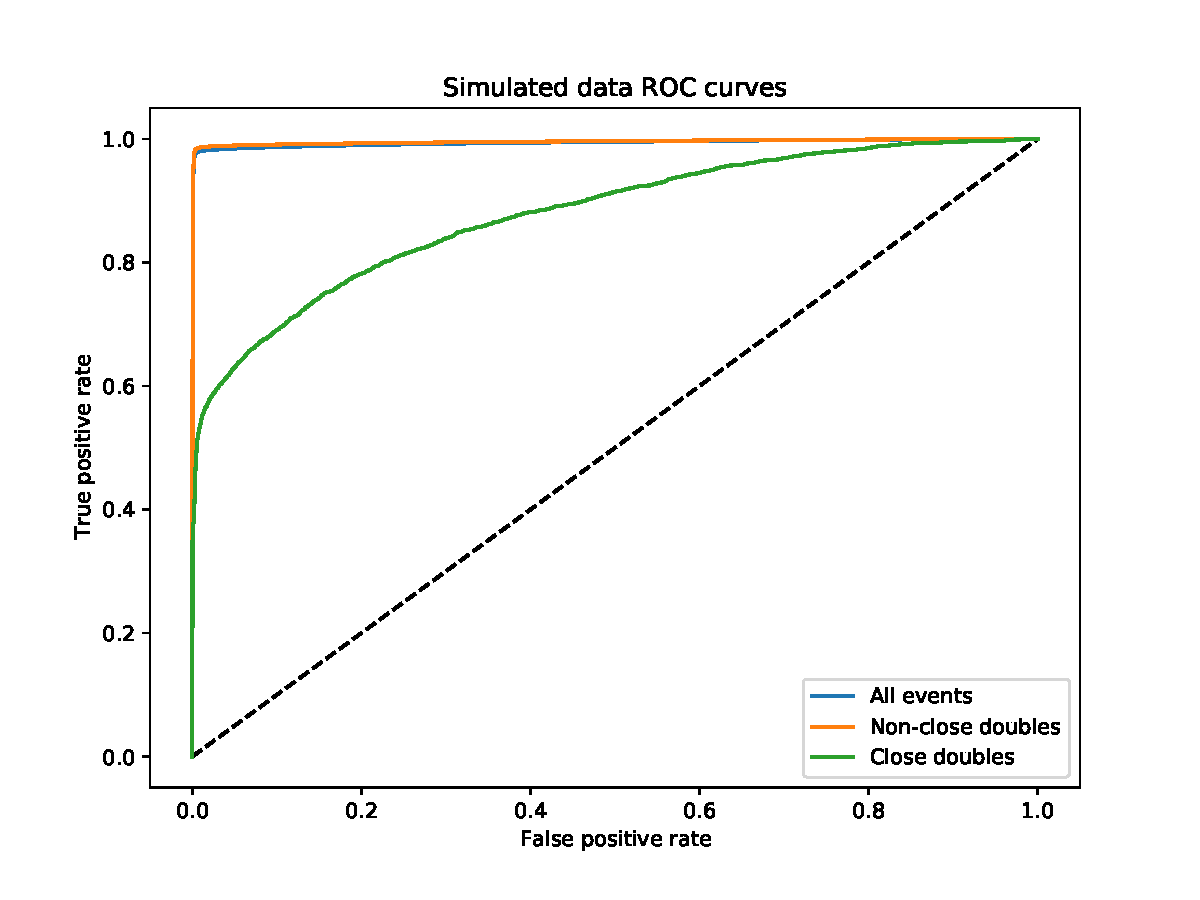
\includegraphics[width=0.8 \textwidth]{chapters/results/figures/roc_simulated.pdf}
\caption[Titletext]{generic text}\label{fig:roc_simulated}
\end{figure}

\subsection{Experimental data}

\section{Regression}
On data already classified, we attempt to predict the energy of the events and the position of origin for
the electrons. Because there is a travel distance between the ejection site and the scintillator array,
the positions aren't necessarily the locations of the highest-intensity pixels in the detector images.
\subsection{Simulated data}
\subsubsection{Position - Single electron}
\begin{table}
\centering
\caption{
Mean R2-scores for regresson of positions of origin, on single events in simulated data, using multiple models. 
Error estimates are the standard deviation in results from k-fold cross-validation 
with $K=5$ folds.
}
\label{tab:regression-simulated-single-position-r2}
\begin{tabular}{lllll}
\toprule
                                           Linear &                                               Dense &                                       Convolutional &                                    Pretrained VGG16 &                                              Custom \\
\midrule
 $\underset{\num{+- 3.664e-03 }  }{\num{ 0.8 } }$ &  $\underset{\num{+- 8.185e-04 }  }{\num{ 0.991 } }$ &  $\underset{\num{+- 2.401e-04 }  }{\num{ 0.997 } }$ &  $\underset{\num{+- 6.864e-03 }  }{\num{ 0.884 } }$ &  $\underset{\num{+- 2.335e-04 }  }{\num{ 0.999 } }$ \\
\bottomrule
\end{tabular}
\end{table}

\subsubsection{Energy - Single electron}
\begin{table}
\centering
\caption{
Mean R2-scores for regresson of energy values, on single events in simulated data, using multiple models. 
Error estimates are the standard deviation in results from k-fold cross-validation 
with $K=5$ folds.
}
\label{tab:regression-simulated-single-energy-r2}
\begin{tabular}{lllll}
\toprule
                                             Linear &                                               Dense &                                                 CNN &                                          Pretrained &                                              Custom \\
\midrule
 $\underset{\num{+- 3.691e-02 }  }{\num{ 0.936 } }$ &  $\underset{\num{+- 3.364e-02 }  }{\num{ 0.938 } }$ &  $\underset{\num{+- 3.282e-02 }  }{\num{ 0.937 } }$ &  $\underset{\num{+- 1.945e-02 }  }{\num{ 0.893 } }$ &  $\underset{\num{+- 3.103e-02 }  }{\num{ 0.944 } }$ \\
\bottomrule
\end{tabular}
\end{table}

\subsubsection{Position - Double electron}
\begin{table}
\centering
\caption{
Mean R2-scores for regresson of positions of origin, on double events in simulated data, using multiple models. 
Error estimates are the standard deviation in results from k-fold cross-validation 
with $K=5$ folds.
}
\label{tab:regression-simulated-double-position-r2}
\begin{tabular}{lllll}
\toprule
                                             Linear &                                               Dense &                                                 CNN &                                         Pretrained &                                              Custom \\
\midrule
 $\underset{\num{+- 5.796e-03 }  }{\num{ 0.364 } }$ &  $\underset{\num{+- 1.809e-03 }  }{\num{ 0.471 } }$ &  $\underset{\num{+- 2.394e-03 }  }{\num{ 0.473 } }$ &  $\underset{\num{+- 1.079e-02 }  }{\num{ 0.37 } }$ &  $\underset{\num{+- 6.812e-04 }  }{\num{ 0.489 } }$ \\
\bottomrule
\end{tabular}
\end{table}

\subsubsection{Energy - Double electron}
\begin{table}
\centering
\caption{
Mean R2-scores for regresson of energy values, on double events in simulated data, using multiple models. 
Error estimates are the standard deviation in results from k-fold cross-validation 
with $K=5$ folds.
}
\label{tab:regression-simulated-double-energy-r2}
\begin{tabular}{lllll}
\toprule
                                             Linear &                                              Dense &                                       Convolutional &                                    Pretrained VGG16 &                                              Custom \\
\midrule
 $\underset{\num{+- 6.501e-02 }  }{\num{ 0.429 } }$ &  $\underset{\num{+- 6.632e-02 }  }{\num{ 0.43 } }$ &  $\underset{\num{+- 5.027e-02 }  }{\num{ 0.433 } }$ &  $\underset{\num{+- 5.308e-02 }  }{\num{ 0.425 } }$ &  $\underset{\num{+- 3.226e-02 }  }{\num{ 0.491 } }$ \\
\bottomrule
\end{tabular}
\end{table}

